\section{Pruebas}

Gracias a la generación automática del esquema OpenAPI, se realizaron pruebas contínuamente del API con la herramienta Insomnia, como se puede observar en la Figura \ref{fig:insomnia-stations-request}. Gracias a esto, se pudieron realizar múltiples pruebas de soluciones, de estructura de la información y de los demás componentes. Ya que fue corroborada la validez de los datos del sistema y que se aseguró la estabilidad del mismo, se procedió a realizar el despliegue del mismo en un ambiente de producción.

\begin{figure}[!ht]
	\centering
	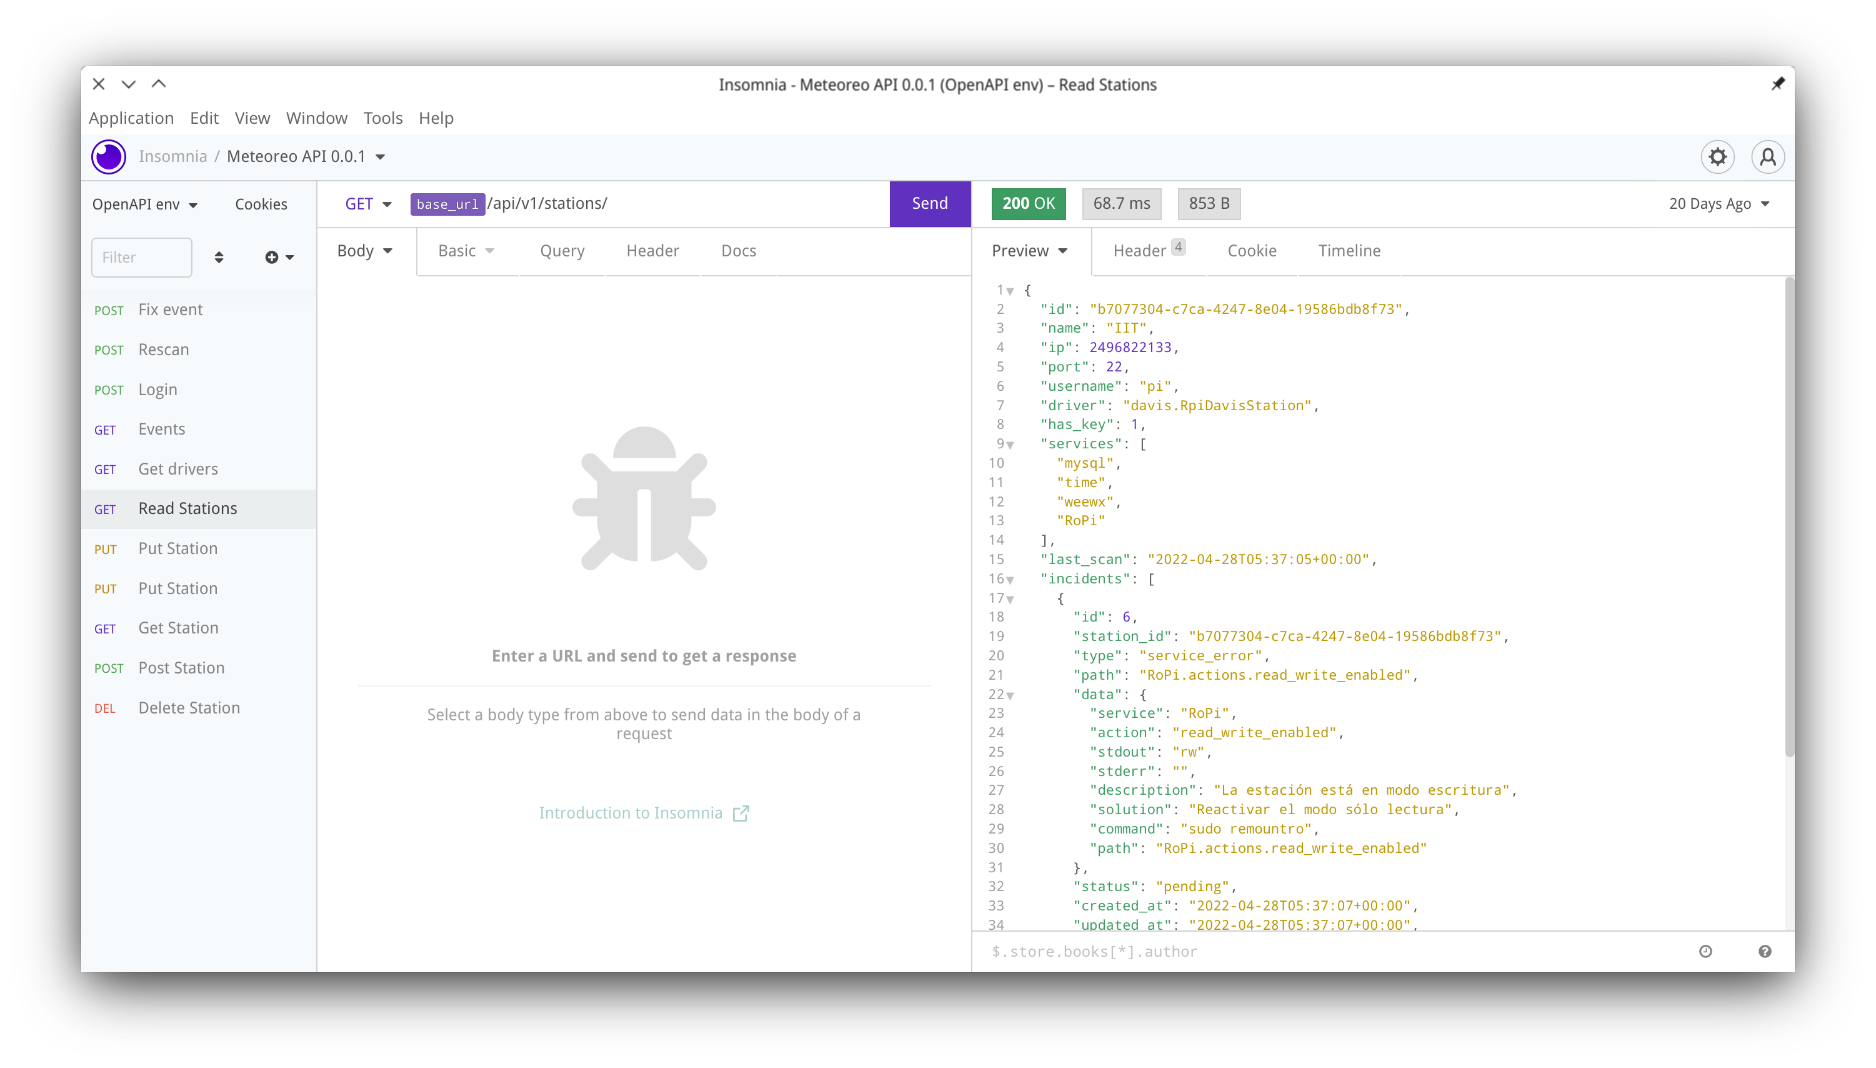
\includegraphics[width=1\linewidth]{images/screenshots/insomnia_stations.png}
	\caption{Solicitud al servidor de pruebas con Insomnia.}
	\label{fig:insomnia-stations-request}
\end{figure}

%TODO: Una última prueba y presentar resultados
